% TODO: Review the dataset section and Diana's comments.
% Your model: Flesh out your own approach, perhaps amplifying themes from the 'Prior lit' section.

% Data: Likely to be very detailed if the datasets are new or unfamiliar to the community, or if familiar datasets are being used in new ways.


\section{Dataset}
% Todo: Add a citation for social gaze about using the AITA subreddit as a proxy for ground truth.

Two datasets were constructed for this project using the Pushshift Reddit Archives \cite{pushshift}, originally collected between 2006 and 2023 through the Pushshift API\footnote{\url{https://github.com/pushshift/api}}. Posts and comments were extracted from two subreddits: (1) \texttt{r/AITAH} and (2) \texttt{r/Anxiety}. For each post, three components were considered: the body the original post written by the author (OP), the most upvoted human-written comment (denoted hc1 in Figure~\ref{fig:pipeline}), and the comment with which the OP engaged the most (hc2). Additional detail regarding data filtering and text preprocessing is provided in Section~\ref{sec:Methods}. Because the dataset predates the public release of GPT‑3.5 in November 2022—and given that large language models (LLMs) only entered widespread public use after early 2023 \cite{liang2025widespread}—all posts and comments in our data can reasonably be considered human-authored.

% Add some comments about why these subreddits were chosen.
\subsection{Subreddit Selection}

The \texttt{r/Anxiety} subreddit is a community dedicated to individuals experiencing anxiety and related mental health challenges. Membership does not require a formal diagnosis or medical documentation, which enables broad analyses from psychosocial perspectives. Posts often center on personal struggles, coping strategies and the impact on daily life.

\medskip The \texttt{r/AITAH} subreddit (short for ``Am I The Asshole'') is a community where users seek judgment on personal dilemmas and social interactions. It has over three million members and covers a wide range of topics, including relationships, family dynamics, workplace conflicts, and personal questions. Users typically describe their situations in detail and ask the community to determine whether they were in the wrong (the ``asshole'') or not. The crowd-sourced social judgments captured in these posts makes \texttt{r/AITAH} a valuable source for examining behaviors and values expressed in digital discussions of personal matters. The crowdsourced verdicts serve as a \textbf{proxy for the ground-truth} judgment of the scenario by humans. This is especially valuable for comparing human responses to the situation against the language model responses under the Goffman's ToF and Rogerian PCT paradigms which serve as signals for "Sycophantic" and "Empathic" behaviors respecitively. 

We construct a balanced dataset of 1000 posts evenly split between the two most common verdicts: ``You're The Asshole'' (YTA) and ``Not The Asshole'' (NTA) directly from the Pushshift Reddit Archives.

Demographic information at the subreddit level is not available. However, research indicates that Reddit users overall are predominantly American (49.9\%), male (67\%), and young (22\% aged 18--29 years; 14\% aged 30--49 years)~\cite{pew-reddit-research,statista-reddit}. While this dataset is not representative of the general population, it reflects a demographic more likely to engage with LLMs for personal queries. This demographic is broadly aligned with the WEIRD (Western, Educated, Industrialized, Rich, Democratic) population, and it must therefore be acknowledged that the results of this study are necessarily constrained to this population.

\section{DeepReflect}\label{sec:deepreflect}
% ~1440 words ≈ ~11–12 paragraphs
% DeepReflect is designed to cater to two broad categories of users:
% 1. Users who frequently interact with LLMs for personal queries. 
% 2. Researchers interested in the large scale analysis and shift in psychosocial paradigms.

\subsection{System Design}
% Design is precise, methodical and shows some flair.

% Add a section on test cases. 
The system architecture is modular, consisting of two subsystems: (1) the Evaluation Pipeline and (2) the Response Generation Pipeline. A high-level overview is presented in Figure~\ref{fig:pipeline}.

Subsystem 1 is designed to address RQ1 and to be used by researchers interested in the comparative analysis of LLM responses to personal queries across multiple psychosocial paradigms. Four psychosocial paradigms have been implemented in this work. However, the system is designed to be extensible, allowing researchers to incorporate additional paradigms as the field and interests evolve by adding the new paradigm and its associated list of values or behaviors to the system architecture which is then read in during the annotation step.

Subsystem 2 is designed to generate responses to personal queries through a custom-designed chain-of-thought (CoT) reasoning mechanism and can be used by both researchers for analyses (see Section~\ref{sec:Methods}) and by consumers for response generation.

\begin{table}[h!]
\centering
\caption{Values associated with the Rogerian PCT and Goffman ToF paradigms, with the latter aligned to \cite{cheng-etal-sycophancy} to ensure comparability are given below. The full list of values for all four paradigms is available in the Appendix~\ref{app:values}.}
\label{tab:values_behaviors}
\begin{tabular}{p{0.35\linewidth} p{0.55\linewidth}}
\hline
\textbf{Paradigm} & \textbf{Values List} \\ \hline
\textbf{Rogerian PCT (Empathy)} & , Emotional Safety, Active Listening, Unconditional Positive Regard, Non-judgmental Acceptance \\[6pt]
\textbf{Goffman ToF (Sycophancy)} & Emotional Validation, Moral Endorsement, Indirect Language, Indirect Action, Accepting Framing \\
\hline
\end{tabular}
\end{table}


\subsubsection{Evaluation Framework}

The evaluation framework consists of the following steps in a pipeline architecture (see Figure~\ref{fig:pipeline}):

\begin{figure}[h!]
    \centering
    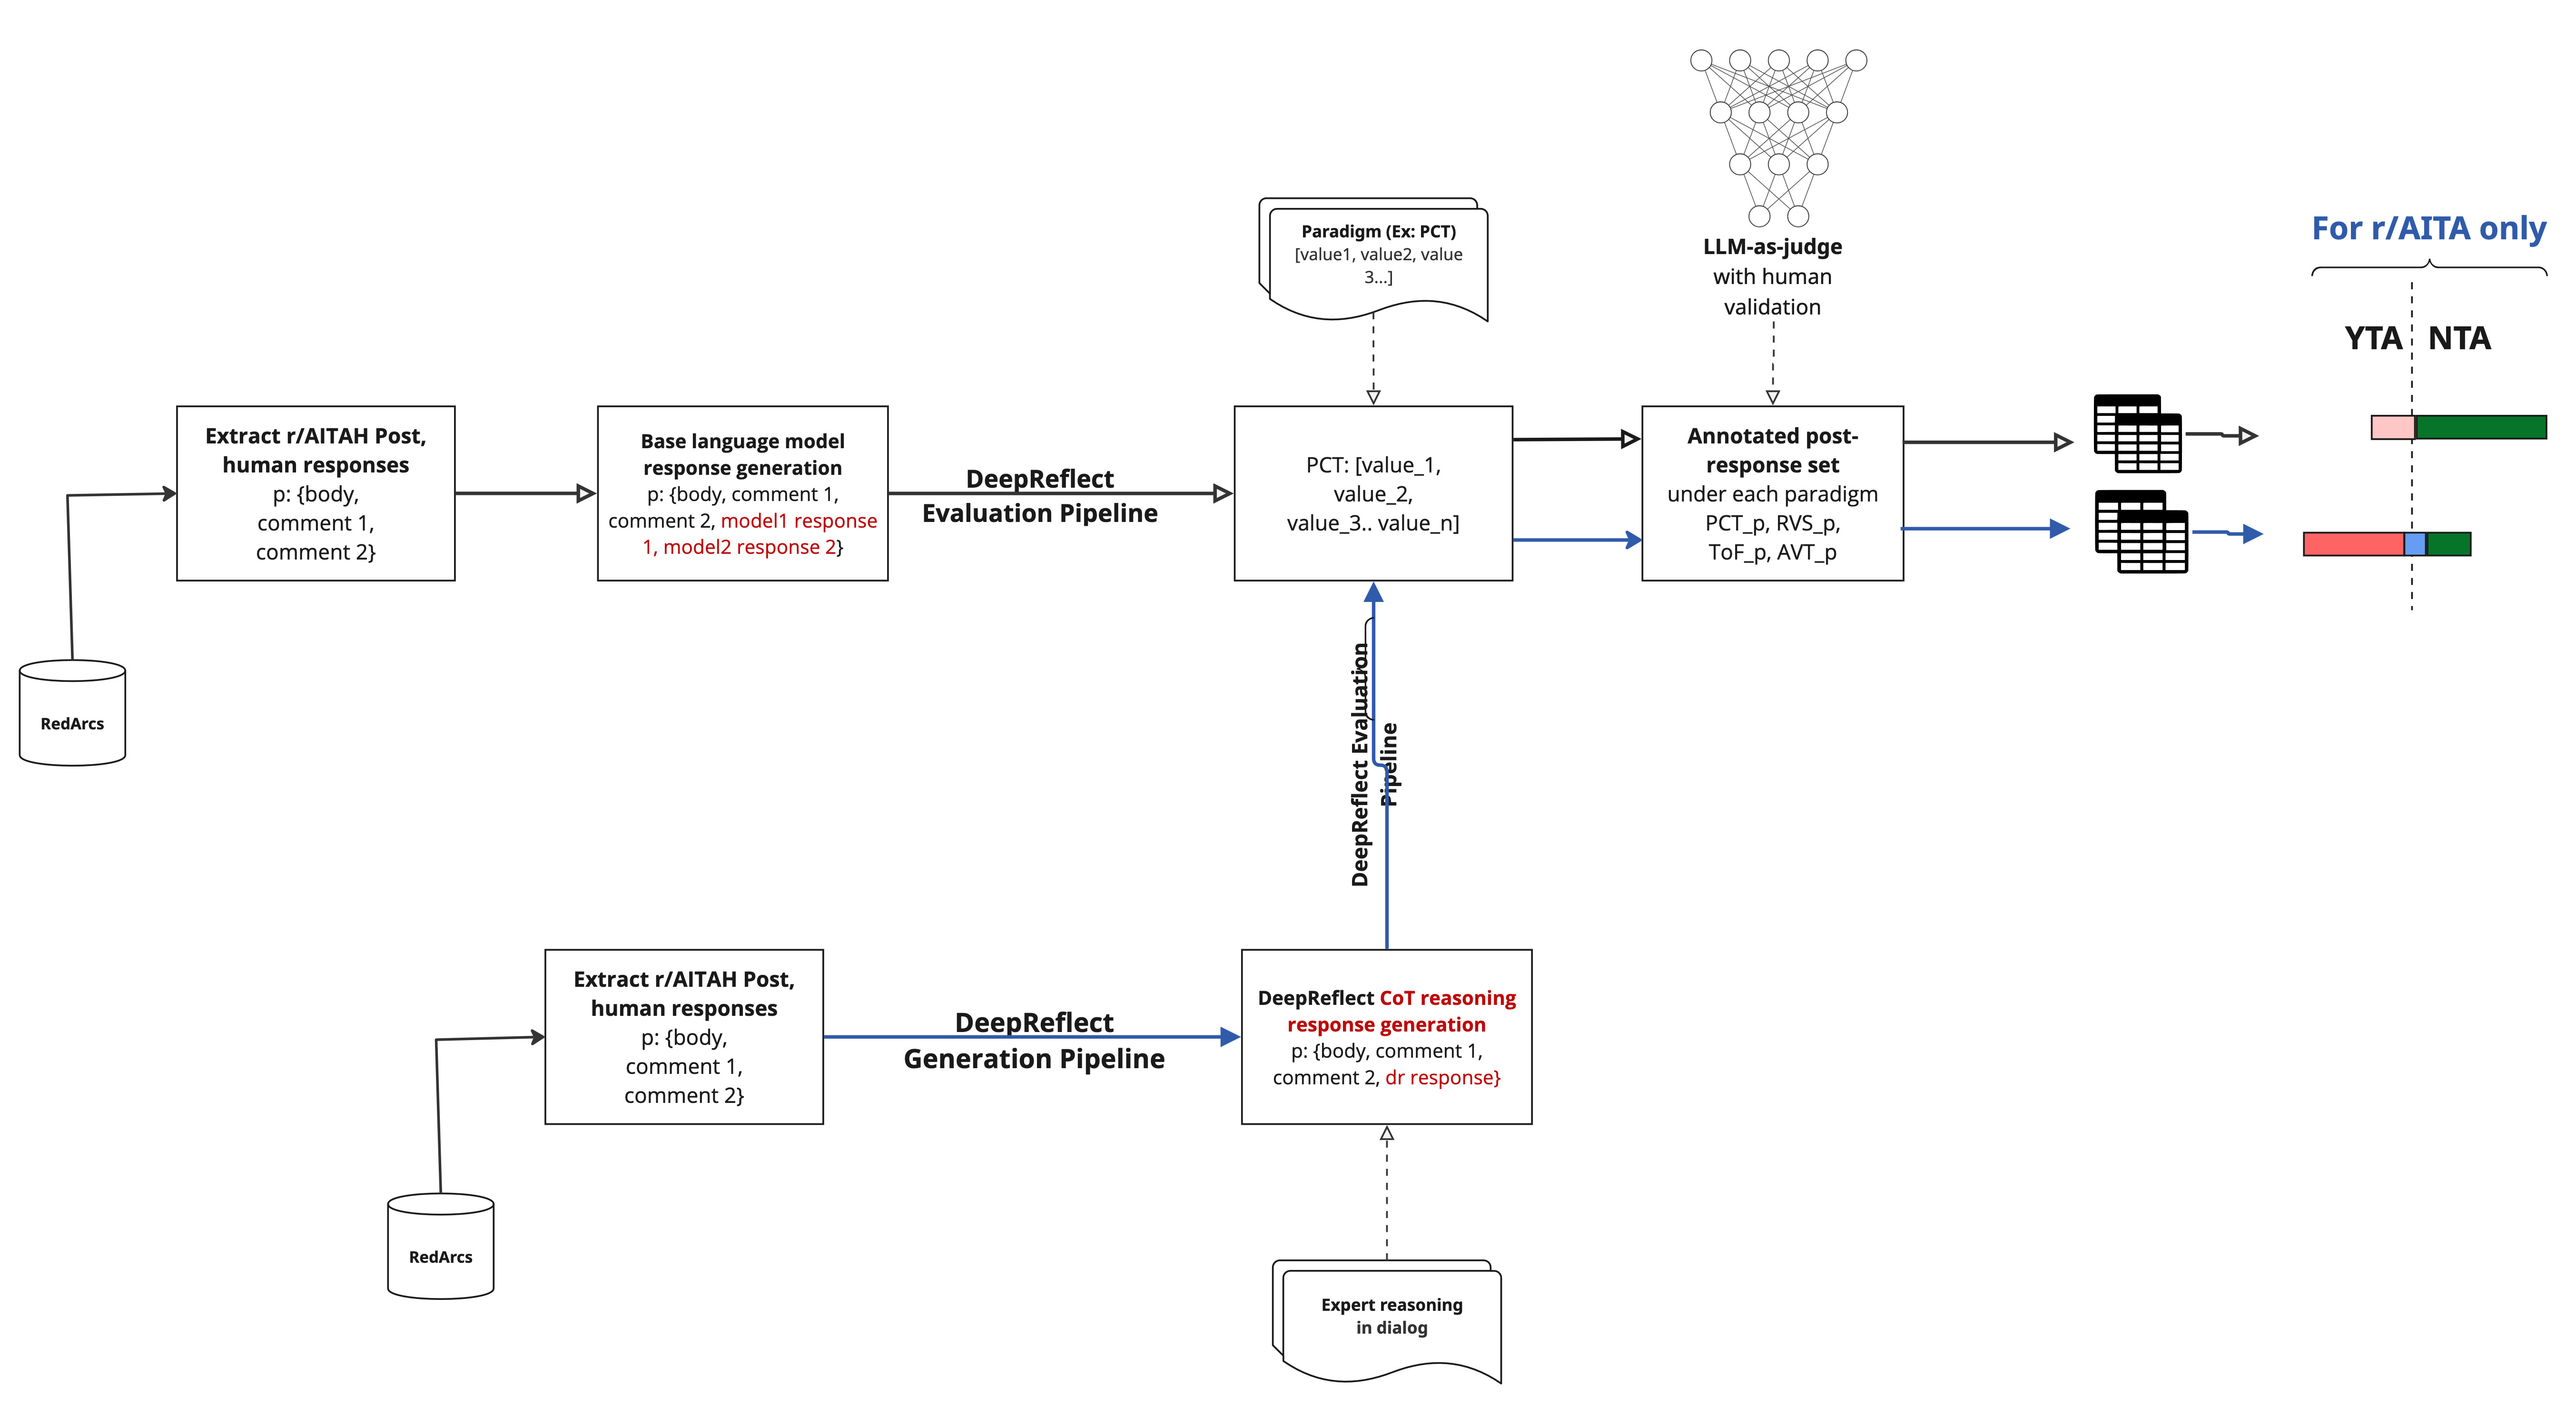
\includegraphics[width=0.98\columnwidth]{Diagrams/pipeline.jpg}
    \caption{Pipeline architecture for DeepReflect.}
    \label{fig:pipeline}
\end{figure}

\begin{enumerate}\label{pipeline_steps}
    \item \textbf{Post and Comment extraction}: The top 1000 posts for two subreddits: (1) \texttt{r/AITAH} and (2) \texttt{r/Anxiety} are extracted from the Reddit Archives dataset. For each post, three components are considered: i. the body the original post written by the author (OP), ii. the most upvoted human-written comment, and iii. the comment with which the OP engaged the most. Additional detail regarding the top post filtering and text preprocessing are provided in Section~\ref{sec:Methods}.
    \item \textbf{Basic Language Model Response Generation}: For each post and body, a baseline response is generated using an API call to the LLM. This response is appended to a dataframe (p in Figure~\ref{fig:pipeline}) containing: (i) The original post title and body (ii) the top most-upvoted human comment, and (iii) the comment the OP engaged the most with (available for 50\% of the posts). The resulting dataset therefore consists of the original post body, paired with two sources of responses to personal queries - human-written and AI responses.
    \item \textbf{Importing Paradigms and the Associated Values}: The following psychosocial paradigms are implemented in this work: (1) RVS, (2) Rogerian PCT, (3) Goffman’s ToF, and (4) Anthropic’s Value Tree (AVT). 
    Each paradigm is associated with a unique list of values or behaviors as described in Section~\ref{sec:Litreview}. The selected paradigms and their associated lists of values are read into the system for annotations in the next step.
    \item \textbf{Feature Extraction and Annotation}: 
    For each post and set of responses, features are extracted and annotated at the sentence level.
    The annotations are made by GPT-4o with the LLM-as-a-judge \cite{zheng-et-al} procedure for the 4 psychosocial paradigms. So, if a sentence exhibits a value or behavior, it is annotated as \textbf{1}, otherwise it is annotated as \textbf{0} for each value under the paradigm. For example, features demonstrating “unconditional positive regard,” a value within Rogerian PCT, are annotated as \textbf{1} for that value; all others are annotated as \textbf{0}.

    For the annotation step, human validation is performed with one expert annotater familiar with the research problem. The human annotater annotates on 100 post-response pairs. This validation along with LLM annotations are used to calculate Cohen's Kappa and accuracy metrics in order to gauge the reliability of the annotations.
    % Cohen's Kappa
    \[
    \kappa = \frac{p_o - p_e}{1 - p_e},
    \]
    \[
    \begin{aligned}
    p_o &= \text{observed agreement (accuracy)} \\
    p_e &= \text{expected agreement by chance}
    \end{aligned}
    \]
    See section~\ref{sec:Methods} for validation metrics.

    \item \textbf{Save dataframe to file}: The resulting annotated data, along with the post and correspondingset of responses are saved to a file.

    \item \textbf{Statistical Analysis}: The annotated dataframe serves as the foundation for subsequent analyses (see Section~\ref{sec:Analysis}), including (i) comparing value distributions in Reddit versus language model responses across the four paradigms, (ii) conducting topical analyses, and (iii) addressing RQs 2 and 3~\ref{sec:RQs} with inter-paradigm correlations.
\end{enumerate}

Note that the standard softmax distribution over a vocabulary of size $V$ for transformer based LLMs with a temperature parameter $T > 0$ that rescales the logits before normalization is: 

\begin{equation}
p_i^{(T)} = \frac{e^{z_i / T}}{\sum_{j=1}^{V} e^{z_j / T}}.
\label{eq:temp-softmax}
\end{equation}

Lower $T$ ($T<1$) sharpens the distribution, making the model more deterministic, while higher $T$ ($T>1$) flattens it, encouraging diversity in the generated responses. For response generations, $T$ is first set to 0 which corresponds to greedy decoding, ensuring fully reproducible results for research and then to $T = 1.0$ to see how responses vary with more stochasticity under more realistic consumer usage conditions.

\subsubsection{DeepReflect Generation Pipeline}
In this subsystem, responses to the post are generated through a custom-designed chain-of-thought (CoT) reasoning mechanism. Instead of relying on standard language model outputs, the framework generates responses that are explicitly guided by reasoning chains derived from \textbf{expert human reasoning in dialog} and transcripts. The expert human transcripts are retrieved from existing literature within Carl Roger's PCT paradigm \cite{rogersgloria} in this instance. See figure ~\ref{fig:rogers_diagram} for details.

\subsection*{Chain-of-Thought Reasoning}

The CoT generation process is formalized as follows:

\[
p_\theta(y \mid x) = \sum_{z} p_\theta(y \mid x, z) \, p_\theta(z \mid x)
\]

where $x$ is the Reddit-based personal query (i.e. a post body), $z$ is the reasoning chain derived from expert human dialog, $y$ is the response generated by DeepReflect and $\theta$ denotes the parameters of the base language model. Here, $p_\theta(z \mid x)$ denotes the probability distribution over reasoning chains given the query, while $p_\theta(y \mid x, z)$ denotes the probability of generating a response conditioned on both the query and reasoning trajectory. 

Conditioning on $z$ separates reasoning from surface realization, allowing responses to be shaped by expert-informed CoT patterns rather than unconstrained next-token prediction.

Thus patterns inherent in the dialog are into the response space. See Figure~\ref{fig:rogers_diagram}.

\begin{figure}[h!]
    \centering
    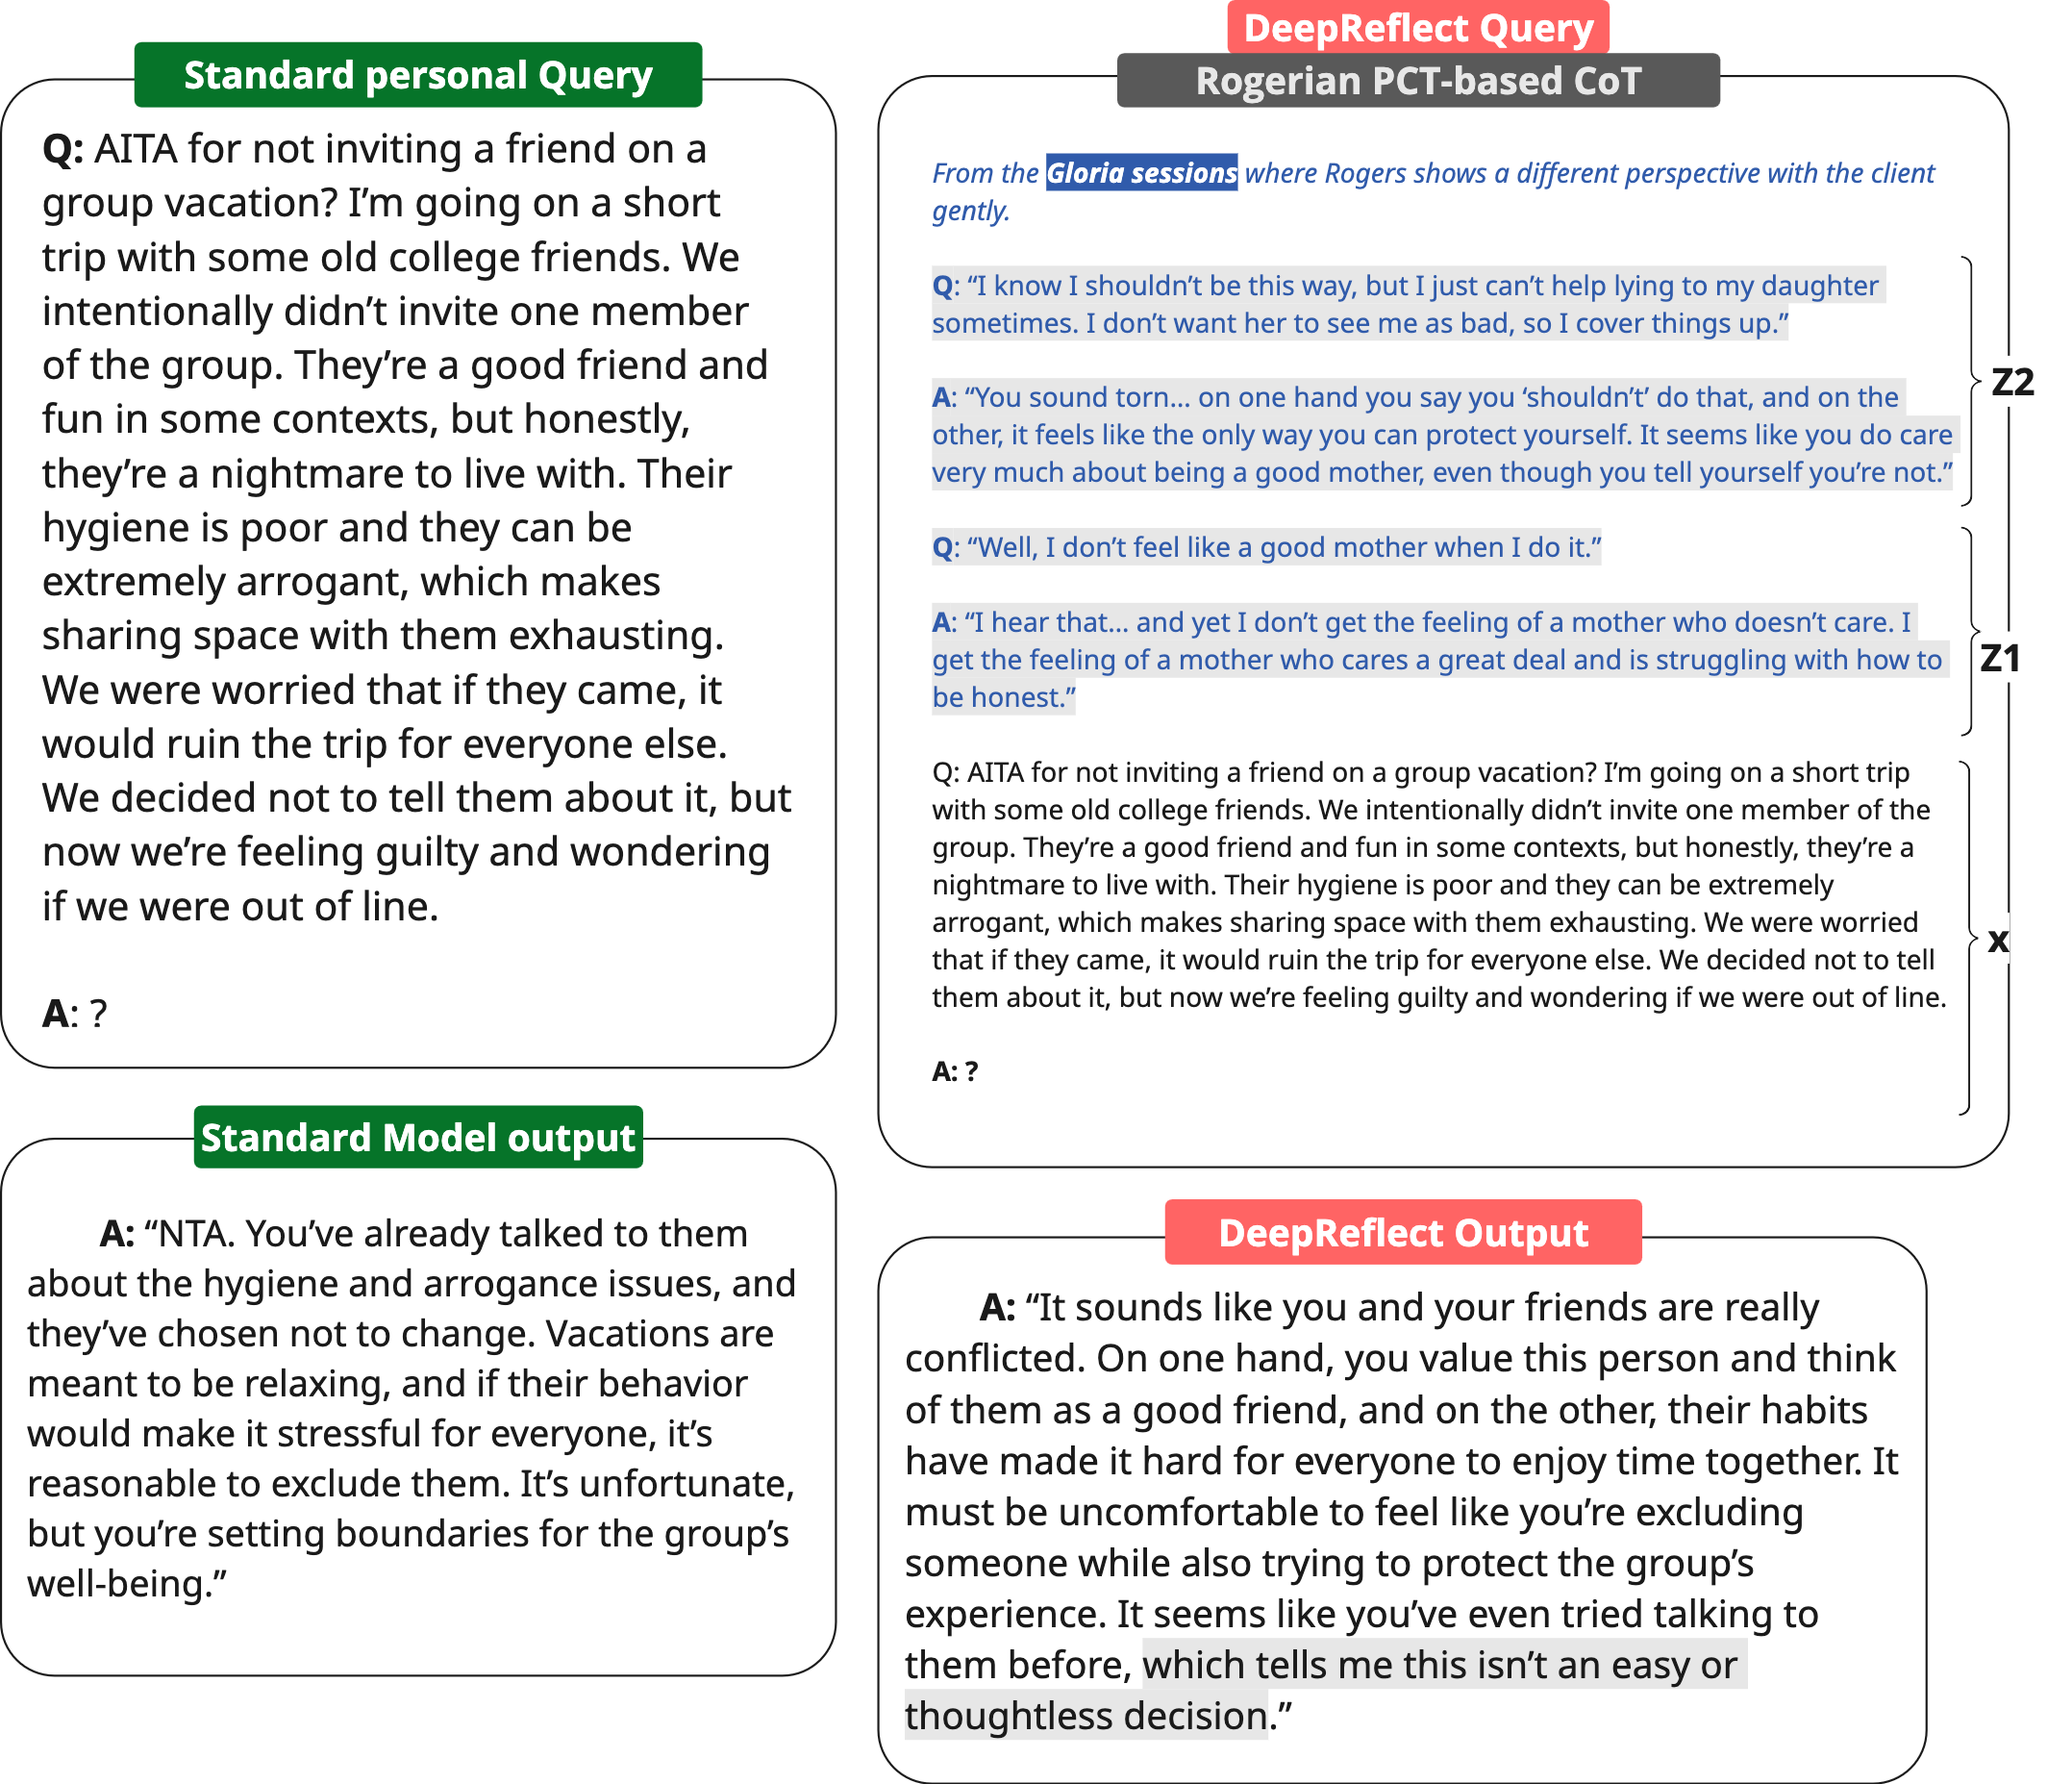
\includegraphics[width=0.98\columnwidth]{Diagrams/Rogers.png}
    \caption{CoT Generation with personal queries embedded in reasoning dialogs retrieved from expert human transcripts. In this case, the dialogs are from Carl Roger's sessions with Gloria (patient) \cite{rogersgloria}. This dialog was selected because it reflects an implicit “NTA” judgment: Gloria expresses guilt about lying to her daughter, and Rogers facilitates exploration of these feelings by gently challenging her self-judgment..}
    \label{fig:rogers_diagram}
\end{figure}

Generated outputs can either be passed through the Evaluation Pipeline for analysis or returned directly in response to a consumer query. In the former case, we evaluate whether PCT-informed CoT reasoning alters verdict distributions (e.g., NTA → YTA or No judgment) and whether such shifts reflect statistically significant divergences in values or principles compared to base LLM responses.

As in the previous section, for evaluation purposes, $T$ is set to both 0 and 1.0 for the CoT generations as well (see Equation~\ref{eq:temp-softmax}).

% GPT 4o vocab size is 199k tokens

% \textcolor{black!60}{Response generations produced on the basis of analyses with Supervised fine-tuning.